\documentclass[11pt]{article}

\usepackage{classDM17}
\usepackage{mathtools}
\DeclarePairedDelimiter\ceil{\lceil}{\rceil}
\DeclarePairedDelimiter\floor{\lfloor}{\rfloor}

\title{Asmt 3: Clustering}
\author{Gopal Menon\\Turn in through Canvas by 2:45pm: \\
Wednesday, March 01}
\date{}

\begin{document}
\maketitle



\section{Hierarchical Clustering (20 points)}

\paragraph{A: (20 points)} 

Single-link clustering will tend to form clusters that are larger. The reason is that when the distance between clusters is the closest distance between parts of two clusters, even if other cluster components are spread out, the closest components will determine whether to merge or not. This can be seen in figure \ref{SLC} with the pink cluster. The opposite effect can be seen in figure \ref{CLC} where the clusters are smaller in the case of the complete-link measure that measures the longest link. The three variants all seem to have done a good job. The points on the top left were separated out by all three methods as part of a cluster. The bottom left and top right points have also been separated out.\\

Both the single-link and complete-link distances will be the easiest to compute through use of a priority queue that stores the distance between pairs of clusters since the queue can be sorted on the shortest or the longest distance. The mean-link computation takes the most time since it has to find the distance between all points in two clusters.

\begin{figure}[!htb]
\centering
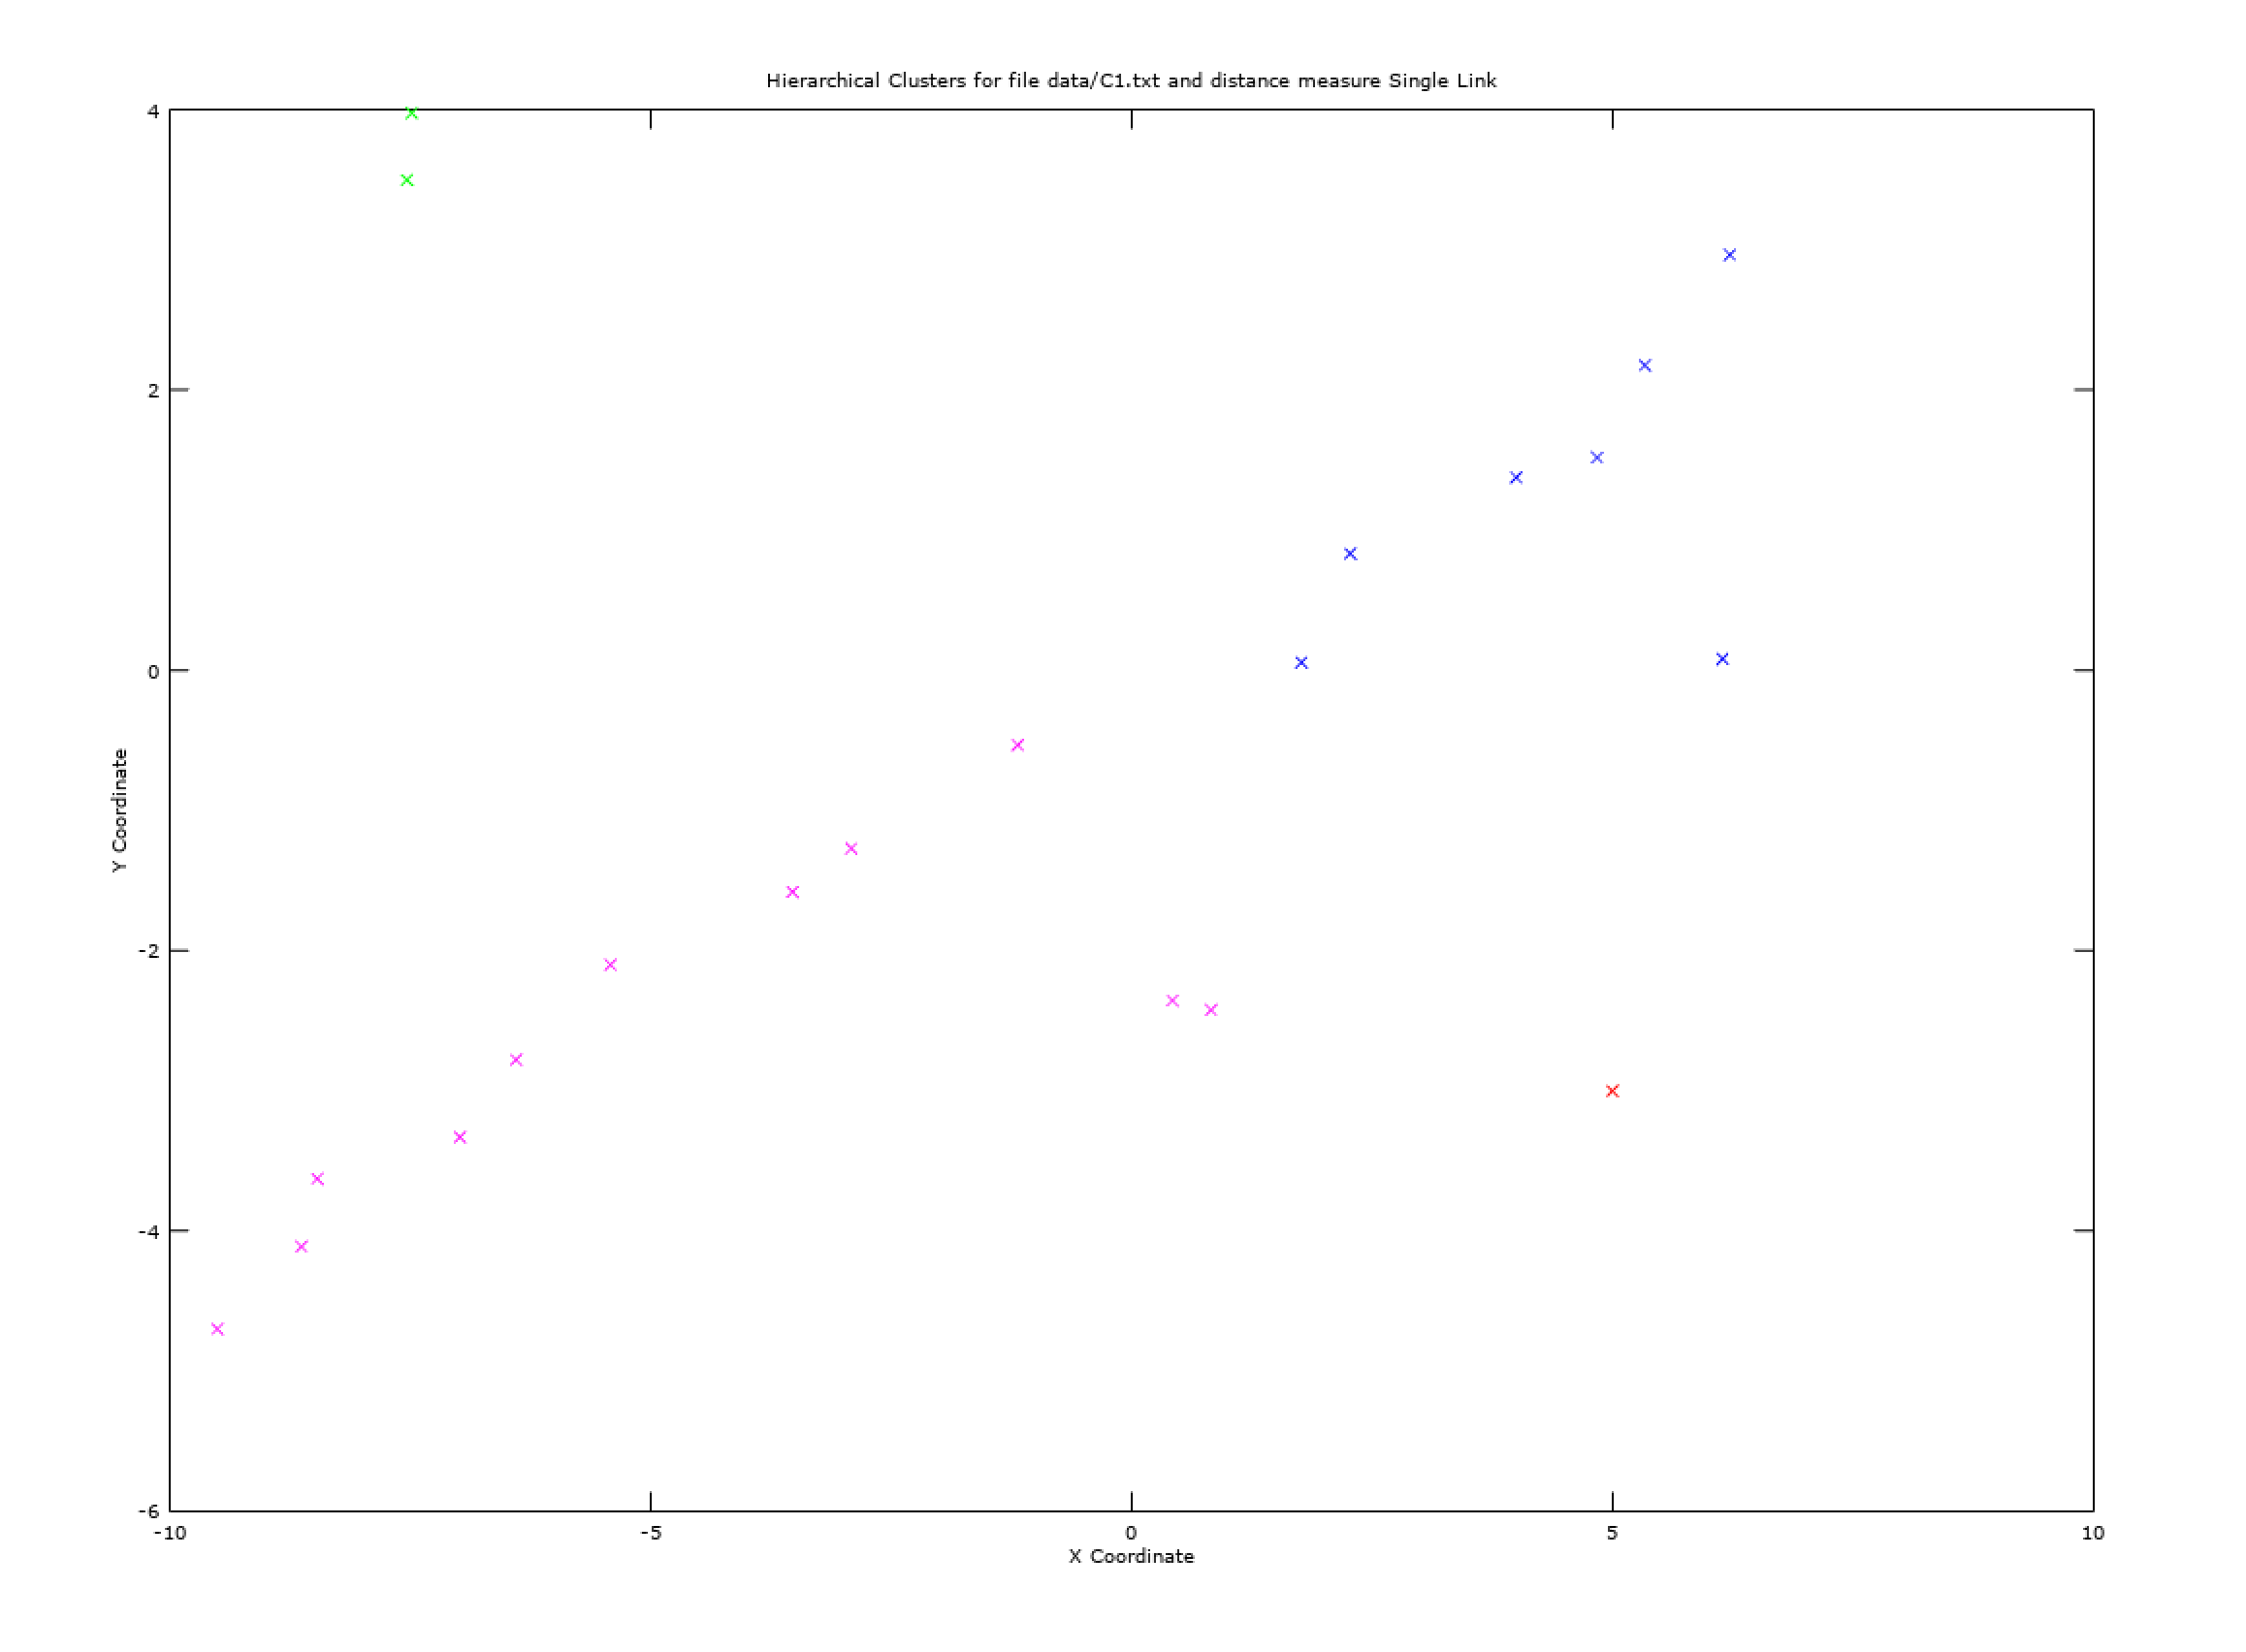
\includegraphics[width=5in]{figures/1ASingleLink.png}
\caption{Single Link Distance Measure Clustering}
\label{SLC}
\end{figure}
 
\begin{figure}[!htb]
\centering
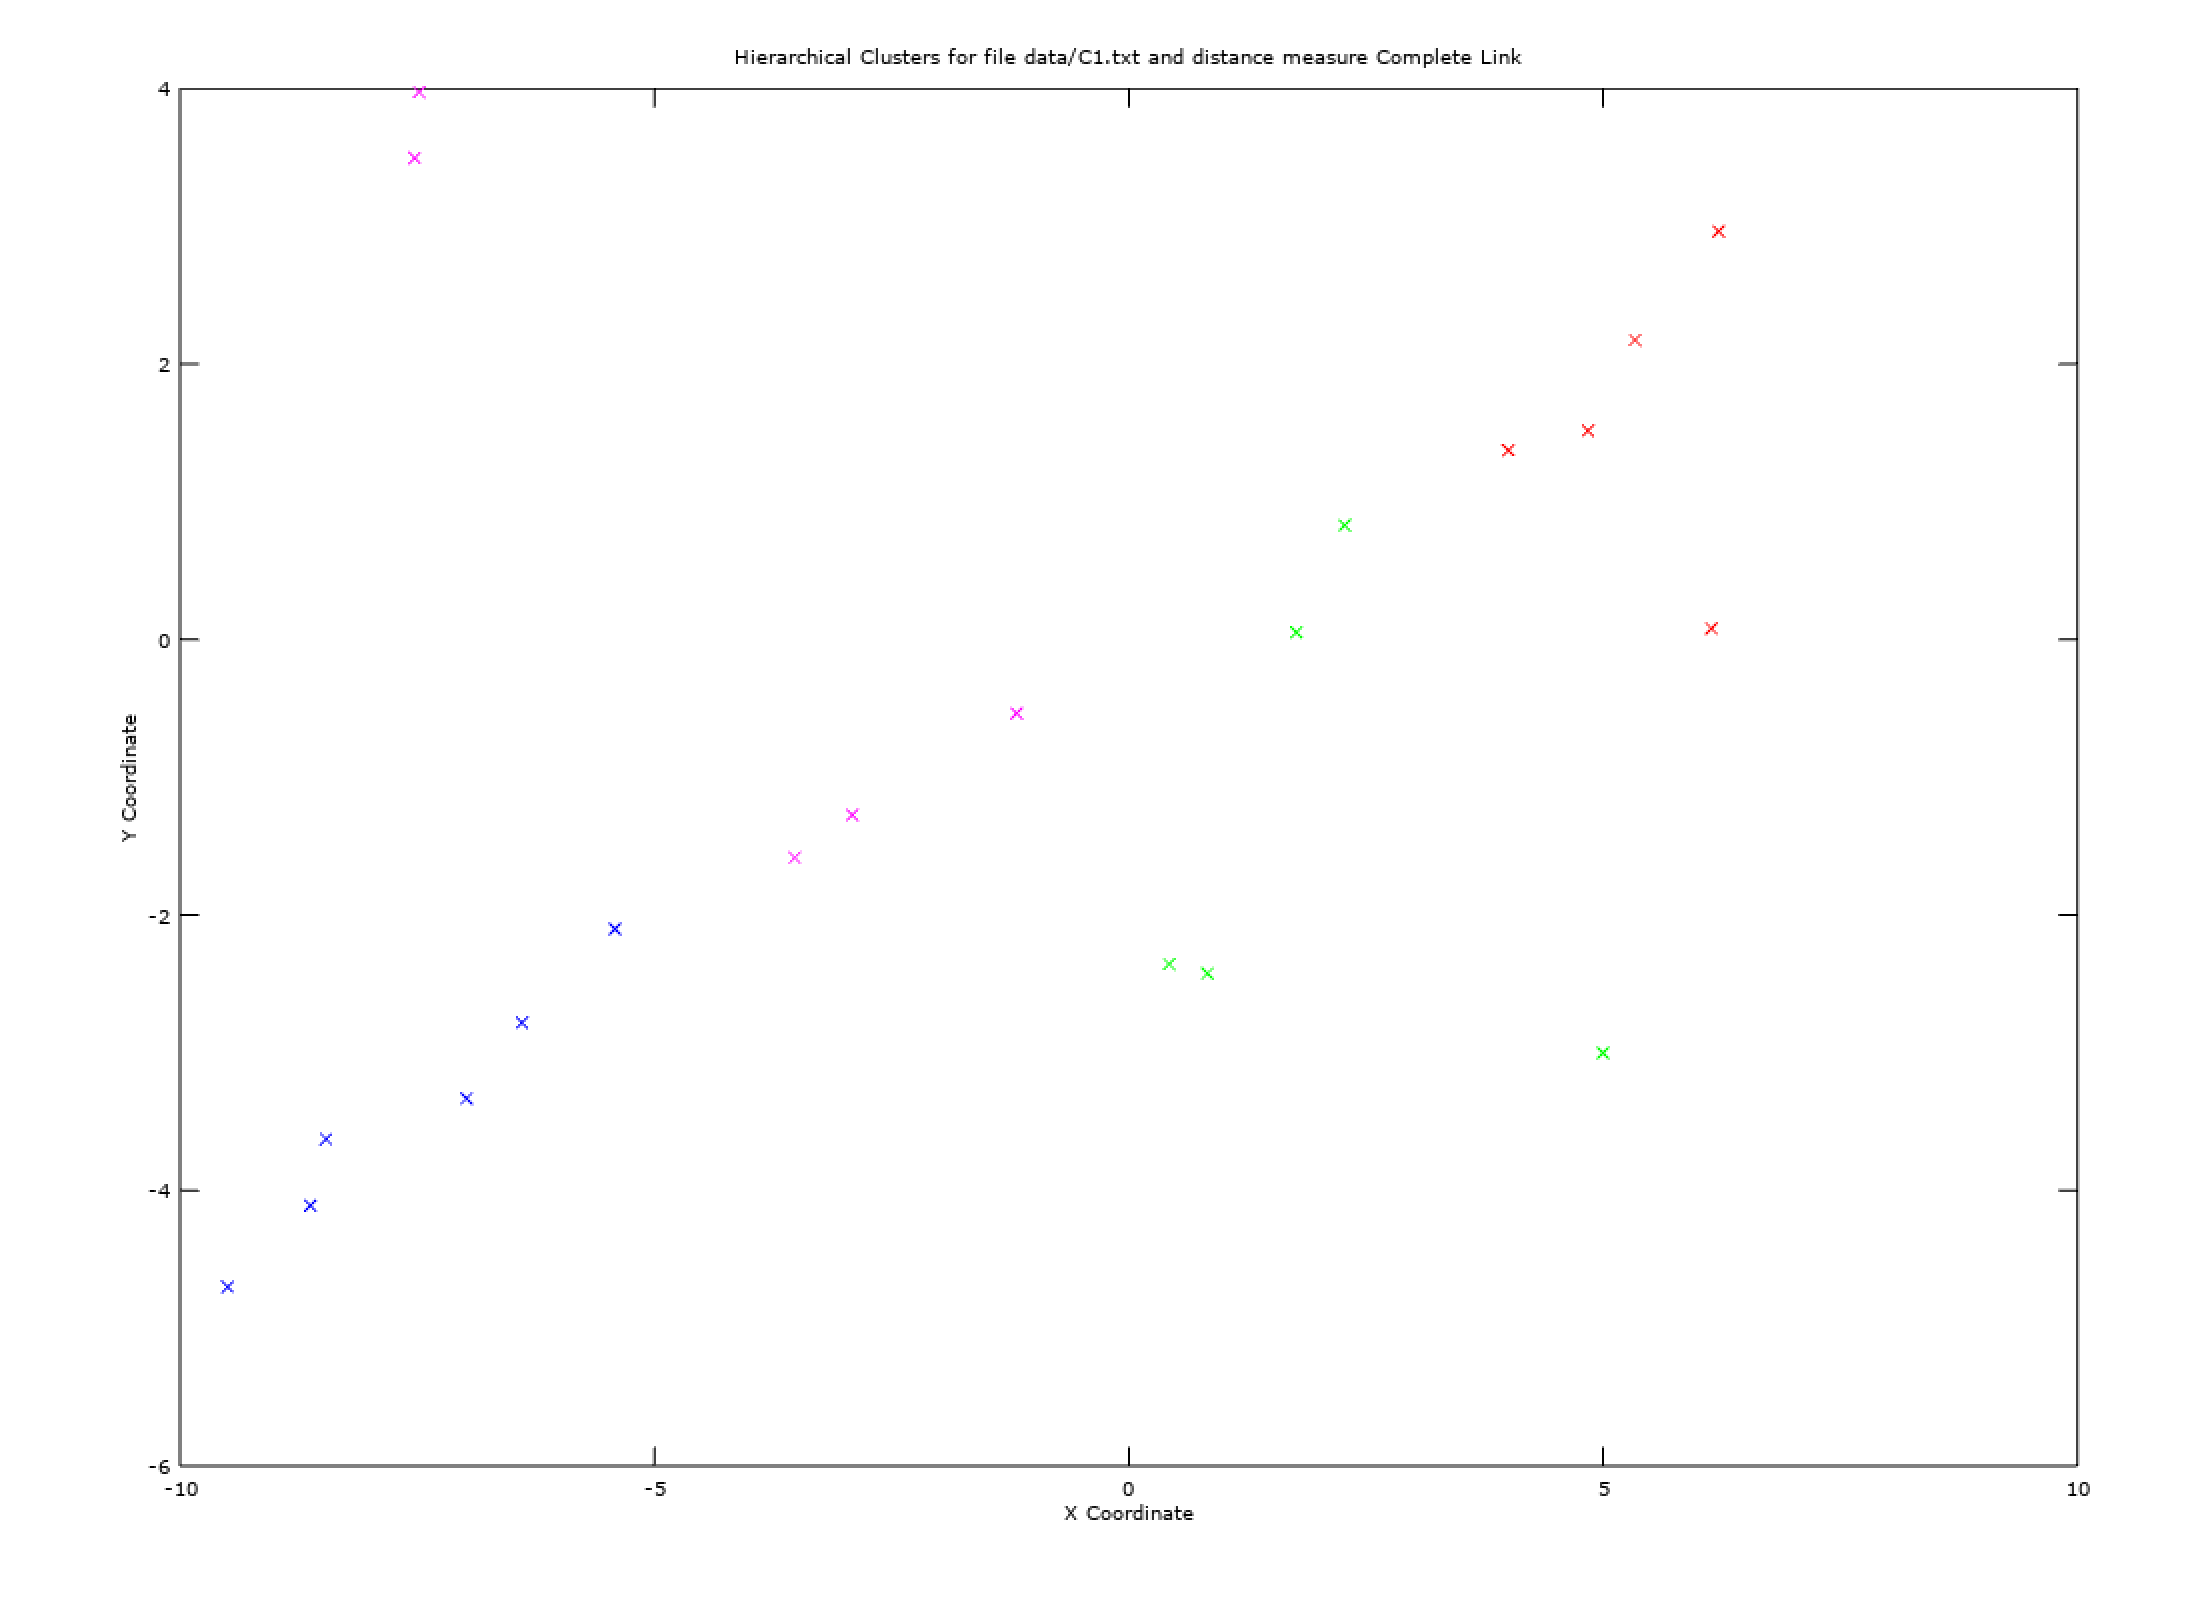
\includegraphics[width=5in]{figures/1ACompleteLink.png}
\caption{Complete Link Distance Measure Clustering}
\label{CLC}
\end{figure}

\begin{figure}[!htb]
\centering
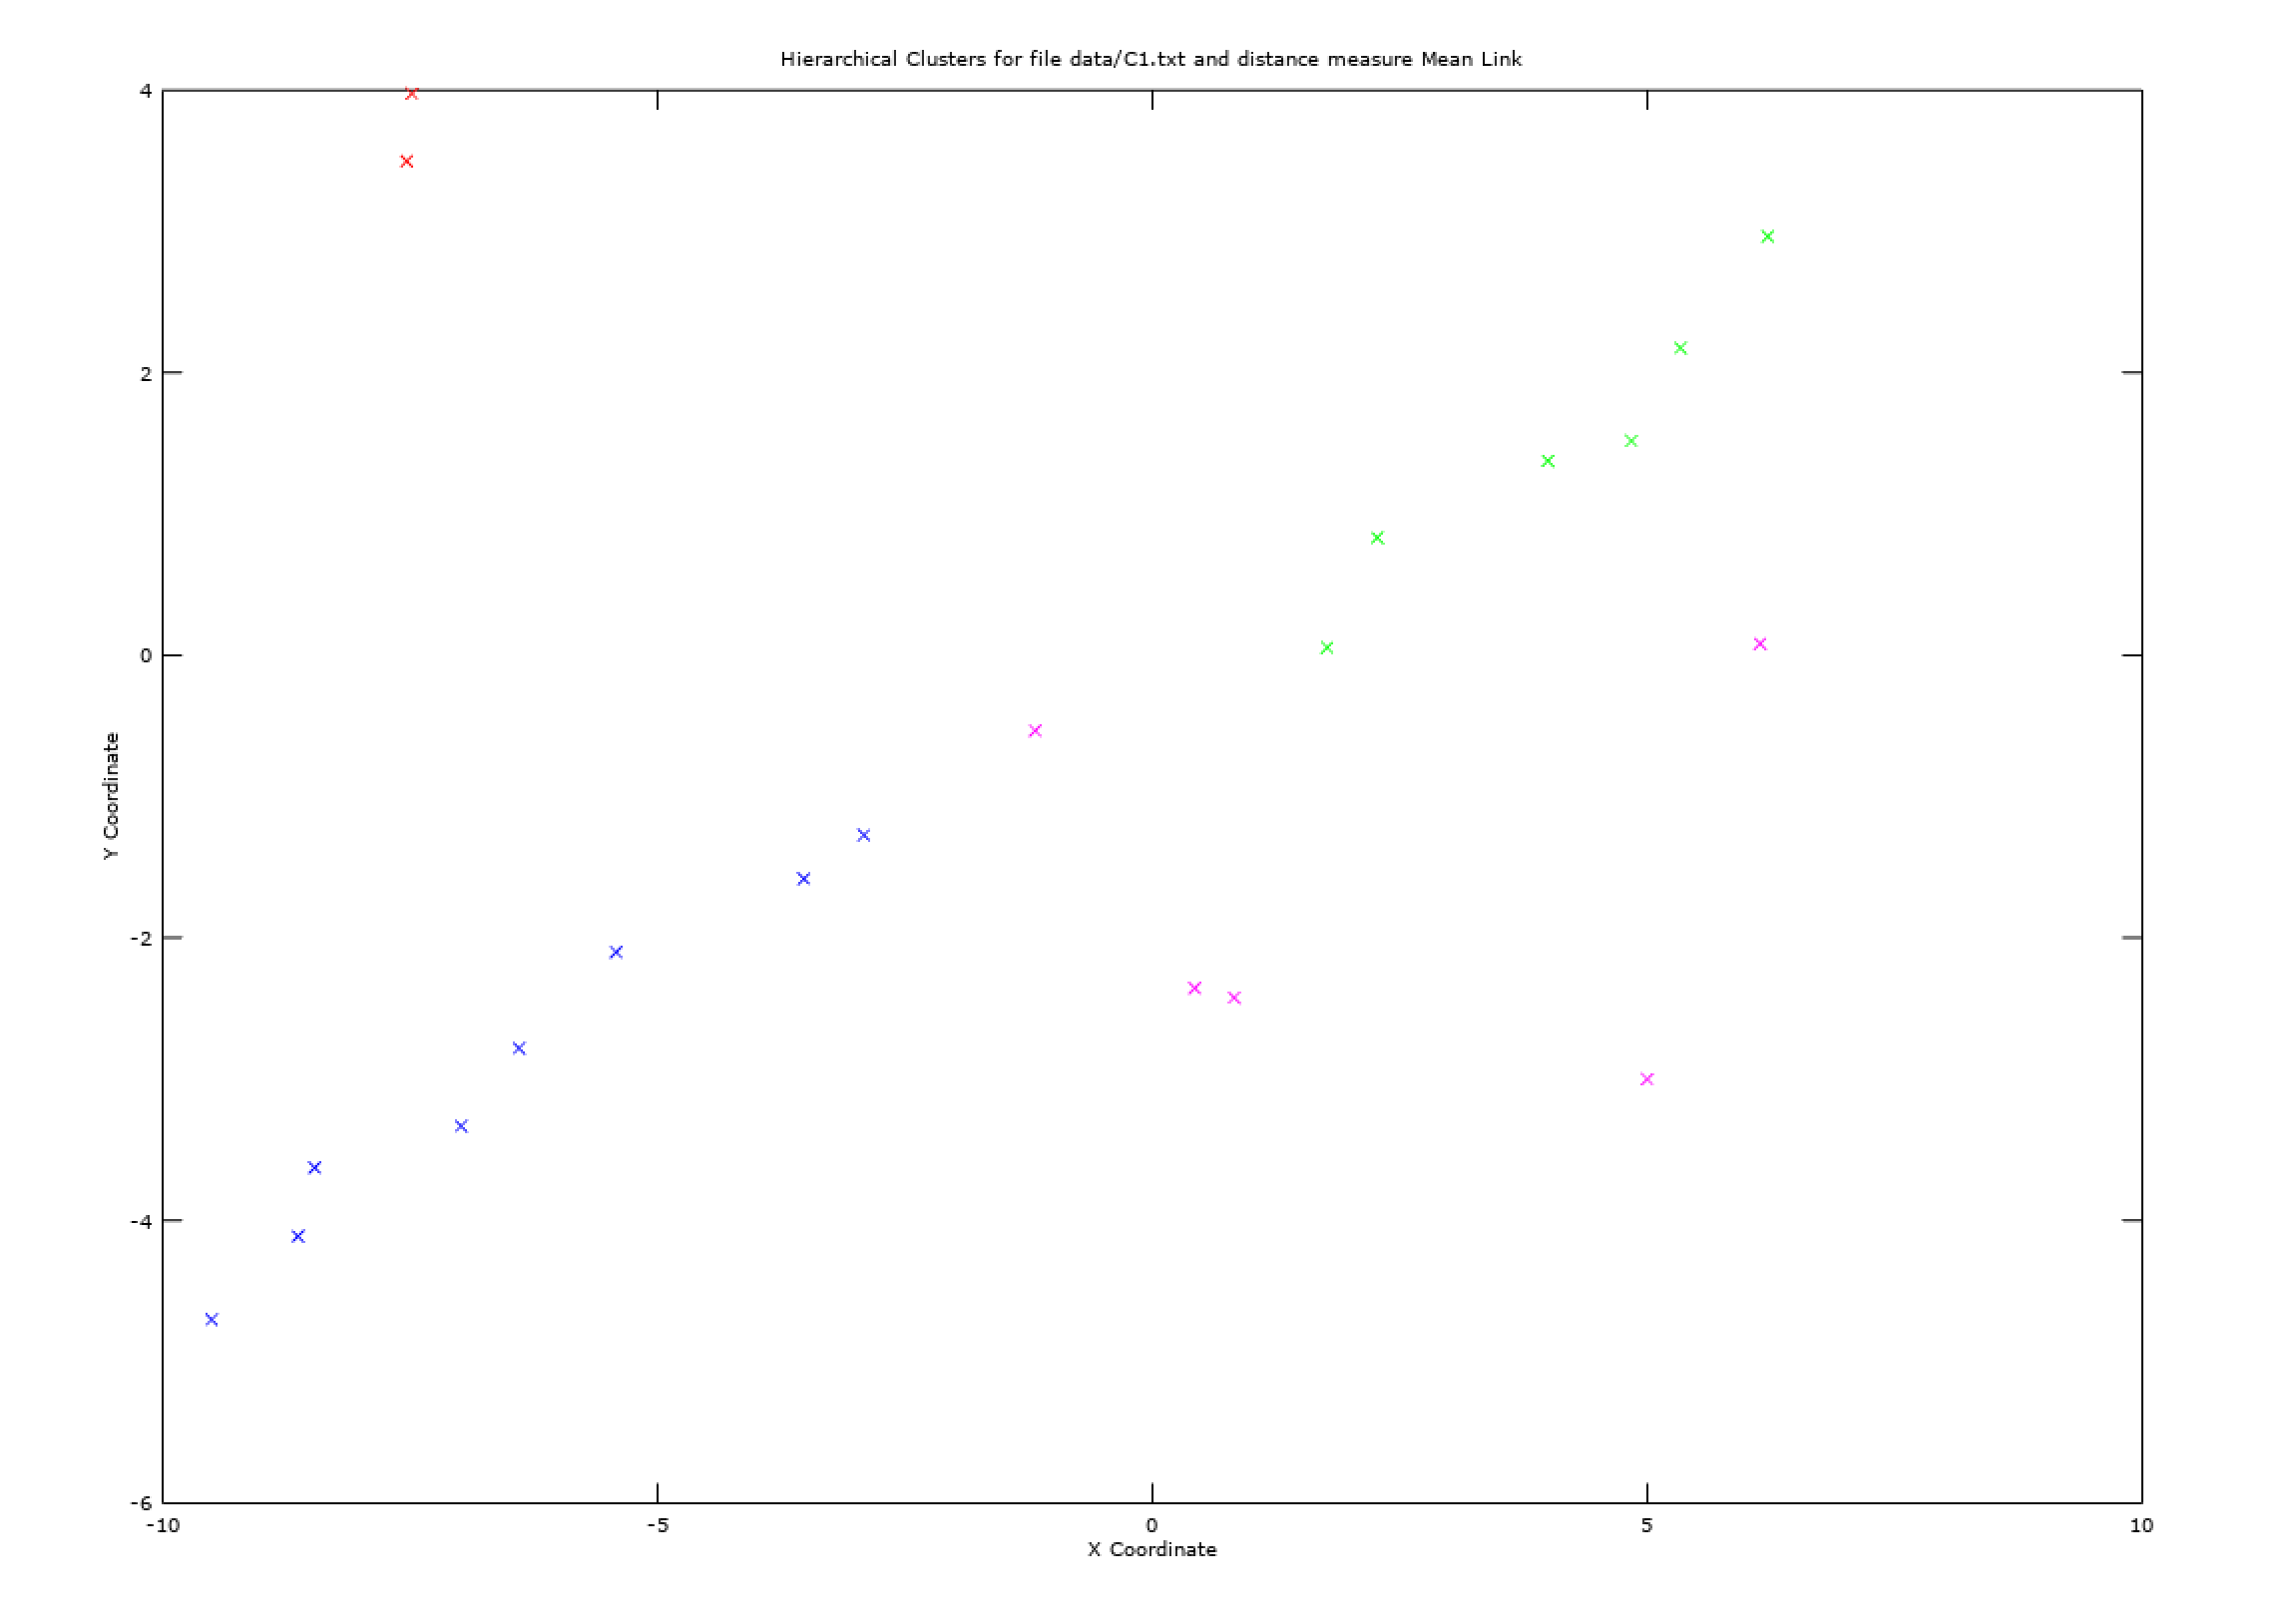
\includegraphics[width=5in]{figures/1AMeanLink.png}
\caption{Mean Link Distance Measure Clustering}
\label{MLC}
\end{figure}
\end{document}
